\section{独立集合遷移問題の ASP 符号化}\label{sec:proposal}

\begin{figure*}[tbp]
  \centering
  \begin{tabular}{ccccccc}
    $t=0$ && $t=1$ && $t=2$ && $t=3$ \\
    \scalebox{0.7}{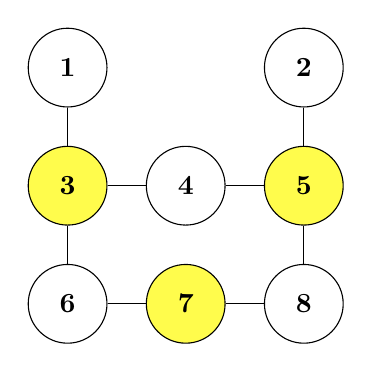
\begin{tikzpicture}[x=1.5cm, y=1.5cm]
  % 設定
  \tikzset{node/.style={circle,draw=black,minimum size=1cm}}
 
  % 色
  \definecolor{yellow}{RGB}{255,251,0}
 
  % 補助線
  % \draw [help lines,blue] (0,0) grid (20,6);
 
  % node %
  \node[node] at (-1,1) (node1) {\textbf{1}};
  \node[node] at (1,1) (node2) {\textbf{2}};
  \node[node, fill=yellow!70] at (-1,0) (node3) {\textbf{3}};
  \node[node] at (0,0) (node4) {\textbf{4}};
  \node[node, fill=yellow!70] at (1,0) (node5) {\textbf{5}};
  \node[node] at (-1,-1) (node6) {\textbf{6}};
  \node[node, fill=yellow!70] at (0,-1) (node7) {\textbf{7}};
  \node[node] at (1,-1) (node8) {\textbf{8}};
 
  \foreach \u / \v in {node1/node3, node2/node5, node3/node4, node3/node6, node4/node5,
    node5/node8, node6/node7, node7/node8}
  \draw (\u) -- (\v);
\end{tikzpicture}
} &
    \lw{$\Rightarrow$} &
    \scalebox{0.7}{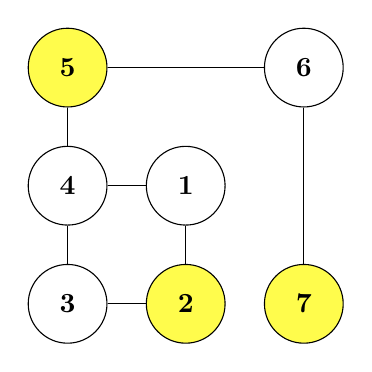
\begin{tikzpicture}[x=1.5cm, y=1.5cm]
  % 設定
  \tikzset{node/.style={circle,draw=black,minimum size=1cm}}
 
  % 色
  \definecolor{yellow}{RGB}{255,251,0}
 
  % 補助線
  % \draw [help lines,blue] (0,0) grid (20,6);
 
  % node %
  \node[node] at (0,0) (node1) {\textbf{1}};
  \node[node, fill=yellow!70] at (0,-1) (node2) {\textbf{2}};
  \node[node] at (-1,-1) (node3) {\textbf{3}};
  \node[node] at (-1,0) (node4) {\textbf{4}};
  \node[node, fill=yellow!70] at (-1,1) (node5) {\textbf{5}};
  \node[node] at (1,1) (node6) {\textbf{6}};
  \node[node, fill=yellow!70] at (1,-1) (node7) {\textbf{7}};
 
  \foreach \u / \v in {node1/node2, node1/node4, node2/node3, node3/node4, node4/node5,
    node5/node6, node6/node7}
  \draw (\u) -- (\v);
\end{tikzpicture}
} &
    \lw{$\Rightarrow$} &
    \scalebox{0.7}{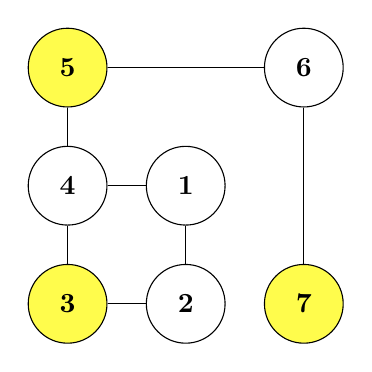
\begin{tikzpicture}[x=1.5cm, y=1.5cm]
  % 設定
  \tikzset{node/.style={circle,draw=black,minimum size=1cm}}
 
  % 色
  \definecolor{yellow}{RGB}{255,251,0}
 
  % 補助線
  % \draw [help lines,blue] (0,0) grid (20,6);
 
  % node %
  \node[node] at (0,0) (node1) {\textbf{1}};
  \node[node] at (0,-1) (node2) {\textbf{2}};
  \node[node, fill=yellow!70] at (-1,-1) (node3) {\textbf{3}};
  \node[node] at (-1,0) (node4) {\textbf{4}};
  \node[node, fill=yellow!70] at (-1,1) (node5) {\textbf{5}};
  \node[node] at (1,1) (node6) {\textbf{6}};
  \node[node, fill=yellow!70] at (1,-1) (node7) {\textbf{7}};
 
  \foreach \u / \v in {node1/node2, node1/node4, node2/node3, node3/node4, node4/node5,
    node5/node6, node6/node7}
  \draw (\u) -- (\v);
\end{tikzpicture}
} &
    \lw{$\Rightarrow$} &
    \scalebox{0.7}{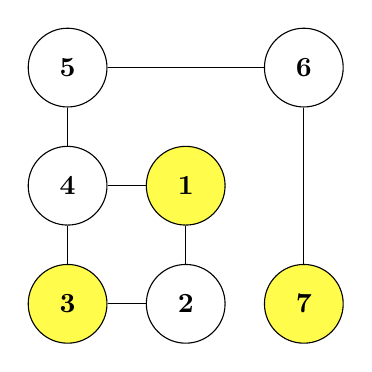
\begin{tikzpicture}[x=1.5cm, y=1.5cm]
  % 設定
  \tikzset{node/.style={circle,draw=black,minimum size=1cm}}
 
  % 色
  \definecolor{yellow}{RGB}{255,251,0}
 
  % 補助線
  % \draw [help lines,blue] (0,0) grid (20,6);
 
  % node %
  \node[node, fill=yellow!70] at (0,0) (node1) {\textbf{1}};
  \node[node] at (0,-1) (node2) {\textbf{2}};
  \node[node, fill=yellow!70] at (-1,-1) (node3) {\textbf{3}};
  \node[node] at (-1,0) (node4) {\textbf{4}};
  \node[node] at (-1,1) (node5) {\textbf{5}};
  \node[node] at (1,1) (node6) {\textbf{6}};
  \node[node, fill=yellow!70] at (1,-1) (node7) {\textbf{7}};
 
  \foreach \u / \v in {node1/node2, node1/node4, node2/node3, node3/node4, node4/node5,
    node5/node6, node6/node7}
  \draw (\u) -- (\v);
\end{tikzpicture}
} \\
    スタート状態 &&&&&& ゴール状態
  \end{tabular}
  \caption{コード\ref{code:isrp_fact.lp}に対する遷移系列の例}
  \label{fig:ex_isrp}
\end{figure*}

%----------------------------------------
\lstinputlisting[float=t,caption={%
独立集合遷移問題を表す ASP ファクトの例.},%
captionpos=b,frame=single,label=code:isrp_fact.lp,%
numbers=none,%
breaklines=true,%
columns=fullflexible,keepspaces=true,%
xrightmargin=1zw,% 
xleftmargin=1zw,% 
basicstyle=\ttfamily\scriptsize]{code/isrp_fact.lp} 
%----------------------------------------

%----------------------------------------
\lstinputlisting[float=t,caption={%
マルチショット ASP 解法における独立集合遷移問題の ASP 符号化.},%
captionpos=b,frame=single,label=code:exact1.lp,%
numbers=none,%
breaklines=true,%
columns=fullflexible,keepspaces=true,%
xrightmargin=1zw,% 
xleftmargin=1zw,% 
basicstyle=\ttfamily\scriptsize]{code/exact1_inc.lp} 
%----------------------------------------

ISRP を表す ASP ファクトの例をコード\ref{code:isrp_fact.lp}に示す.
\code{n/1}はグラフの頂点数,\code{e/1}は辺数,
\code{k/1}は独立集合の要素数を表す.
\code{node/1}は各頂点を,\code{edge/2}は各辺を表す.
\code{staer/1}はスタート状態を表すアトムであり,
頂点\code{X}がスタート状態で独立集合に含まれることを表す.
同様に,\code{goal/1}はゴール状態を表す.

コード\ref{code:isrp_fact.lp}で与えられるインスタンスに対する
遷移系列の例を図\ref{fig:ex_isrp}に示す.
$t=0$がスタート状態,$t=3$がゴール状態として与えられる.
この例では,最短で3回の遷移により到達可能である.
各ステップで,組合せ制約および遷移制約を満たしていることがわかる.

マルチショット ASP 解法における ISRP の ASP 符号化を
コード\ref{code:exact1.lp}に示す.
\code{#program}文は,一つのファイルをいくつかの
サブプログラムにわける記述である.
3行目のルールはスタート制約を表している.
7--8行目は組合せ制約を表している.
10--11行目は遷移制約を表している.
15行目はゴール制約を表している.

コード\ref{code:exact1.lp}とは別に,
求解に必須ではないが,探索効率を上げることを期待した
ヒント制約を5個考案した.
\begin{itemize}
  \item \code{distance1} (d1): スタート状態から$t$ステップ後において,
    スタート状態ではトークンが配置されており,かつステップ$t$では
    配置されていない頂点の数は高々$t$個であることを表す.
  \item \code{distance2} (d2): ゴール状態から$t$ステップ前において,
    ゴール状態ではトークンが配置されており,かつステップ$\ell-t$
    では配置されていない頂点の数は高々$t$個であることを表す.
  \item \code{token1} (t1): ステップ$t-1$で頂点\code{X}から頂点\code{Y}
    にトークンが移動したとき,ステップ$t$で任意の頂点\code{Z}から頂点\code{X}
    へトークンが移動することを禁止する制約である.
    この2ステップの遷移は,ステップ$t-1$で
    頂点\code{Z}から頂点\code{Y}へトークンを
    移動させることで,1ステップで再現できることを利用している.
    冗長な動きを制限するヒント制約であるため,longest では使用できない.
  \item \code{token2} (t2): ステップ$t-1$で頂点\code{X}から頂点\code{Y}
    にトークンが移動したとき,ステップ$t$で頂点\code{Y}から任意の頂点\code{Z}
    へトークンが移動することを禁止する制約である.
    この2ステップの遷移は,ステップ$t-1$で
    頂点\code{X}から頂点\code{Z}へトークンを移動させることで,
    1ステップで再現できることを利用している.
    冗長な動きを制限するヒント制約であるため,longest では使用できない.
  \item \code{heu} (h): ASP システムの{\clingo}では,変数選択
    ヒューリスティックを調整するための構文が用意されている.
    これを利用し,遷移系列の序盤では独立集合がなるべく極大になるようにしている.
\end{itemize}

longest では,遷移系列に同じ実行可能解が高々1回しか出現しない制約を加える
必要がある.
本研究では,「任意の2つのステップにおいて,
独立集合に含まれる頂点がすべて同じにはならない」
ことを表す制約を追加した.
